% -----------------------------------------------------------------------------
%                           Background
% -----------------------------------------------------------------------------
\newpage                                                   \chapter{Background}

%------------------------------------------------------------------------------
\section{                  Binaural Audio                                     }

Three-dimensional audio systems render sound images around a listener by using
either headphones or loud speakers [2]. In the case of 3D audio systems based
on headphones, the 3D audio cues to localize a virtual source can be perfectly
reproduced at the listener’s eardrums because the headphones isolate the
listener from external sounds and room reverberations.  There exist systems that
are capable of producing binaural audio to a user using stereo speakers in an
open environment with the aid of head track ing webcams [3]. Either of these
systems are able to perfectly calibrate sound placement and create an
experience that provide the user with the perception that sound is travelling
around them.


Previous work  have explored binaural audio as positional cues in navigation
applications while the gaming industry rely on these interfaces to enhance the
user experience.


\begin{figure}[h]
  \centering
  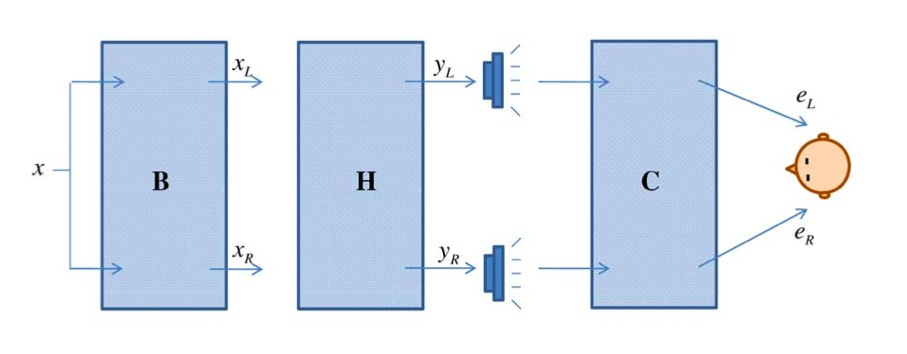
\includegraphics[width=1\textwidth]{images/binaural_diagram.jpg}
  \caption{Schematic of a binaural audio system}
\end{figure}


This paper describes a system that supports a new conceptual model of interface
mapping in 3D space. Using binaural audio as the mechanism, novel features are
discussed that provide information to the user in terms of spatial at-tenuation,
audio structural survey of content on the web, accurate positional audio
feedback, and an audible progress indicator.  These new features can improve
both the user’s comprehension of content presented to them while provid-ed with
cues to assist recall of information.


Human auditory localization has been studied extensively ~\cite{
yost1987directional, blauert1997spatial}. Humans are especially adept at
localizing sounds in three dimensions. Consider a sound source to the left of a
listener.  Sounds from the source arrive at the left ear first, and a short time
after reach the right ear.  The amplitude of the left ear sound will be
attenuated due to head shadowing.


The predominant audiotory cues for determining whether a sound is coming from
the left or right directions are the  interaural intensity differences and the
interaural time differences. Humans are also adept at identifying sound position
that are in front of or behind them, along with estimating the sound source's
elevation.  This is possible because the incident sound waves interact with the
torso, head, external ear (pinna) prior to arriving at the inner ear.


The directional dependent filtering to each of a subject's ears can be expressed
as a frequency response, called a head related transfer function (HRTF), and
thus a pair of HRTFs describe how sound from one location reaches the two ears.
HRTFs are usually measured using human subjects or dummy-head microphones which
consist of response pairs for the left an right ears corresponding to a large
number of source positions surrounding the head.


\begin{figure}[h!]
  \centering
  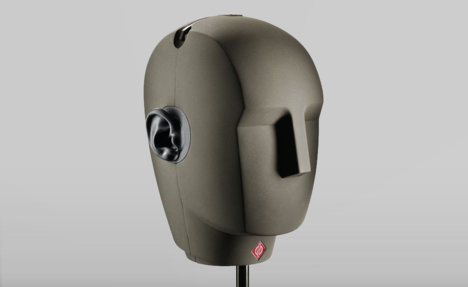
\includegraphics[width=1\textwidth]{images/binaural_mic.png}
  \caption{Binaural microphone with exact dimension and density as human head}
\end{figure}


There are two regions of interest when considering source locations of sound.
When the sound is close to the head, the spherical curvature of the incident
sound waves cause the HRTFs to change qualitatively as a function of distance,
but at moderate distances, the incident waves can be considered planar. At
extreme distances, humans are only capable to process auditory cues that only
depend on the sound sources volume.

Given that humans are capable of processing sound signals to place the audio
source in space, a binaural spatializer can then be implemented to simulate the
auditory experience of one or more sound sources arbitrarily located around a
listener.  The general idea is reproduce the acoustical signals at the two ears
that would occur normally in a natural listening situation.

This process is accomplished by convolving each source signal with a pair of
HRTFs corresponding to the sound sources intended location.  The resulting
signal is presented to the user through headphones.



%------------------------------------------------------------------------------
\section{                  Current Solutions                                  }

\subsection{                  Transaural Audio                                }

Transaural audio is a method used to deliver signals to the ears of a listener
using stereo loudspeakers. The idea is to filter the binaural signal such that
the subject can process the subsequent stereo representation as a binaural
signal.  This technique was first put into practice by Shroeder and Atal
~\cite{ schroeder1963computer, schroeder1970digital }. Song et al. demonstrated
how computer vision techniques could be applied to the field of Transaural
Audio. By tracking a subject's head, the computer can recalculate the HRTFs
necessary for the sound, as well as reposition the sound sources relative to the
subject to provide an adaptive 3D audio system ~\cite{song2010personal}.



%------------------------------------------------------------------------------
\section{                  Research Domain                                    }
\subsection{                  Audio Used for Analytics                        }
\subsection{                  Audio Used for Interfaces                       }


\section{                  Our Approach                                       }





\section{                  Notifications                                      }

The essence of any event or update to user data is condensened into a
notification.  Current research has explored how notification systems attempt to
deliver current, important information to computer screens.  Many works have
also explored the costs, benefits, and optimal displays of these notifications
from psychological prespectives that overlap with our ability to handle
interruptions and distractions~\cite{McCrickard2003509,
cutrell2001notification}.
